\documentclass[border=4pt]{standalone}
\usepackage{amsmath,amssymb,tikz}
\usetikzlibrary{arrows.meta}
\begin{document}
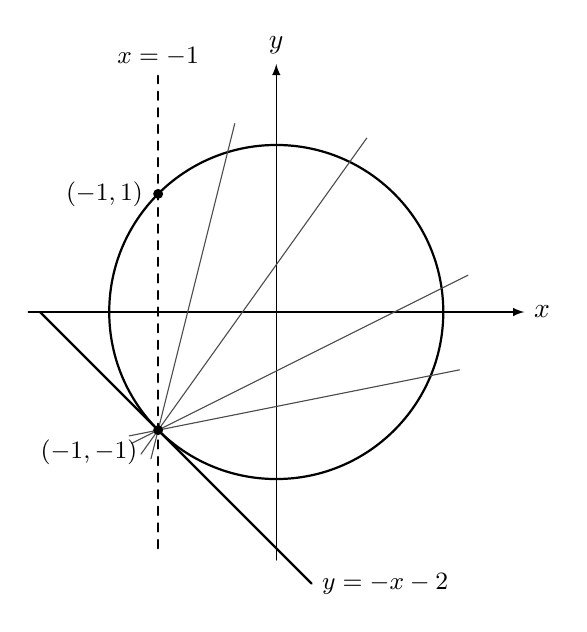
\begin{tikzpicture}[scale=1.5,>=latex,line cap=round]
  \draw[->] (-2.1,0) -- (2.1,0) node[right]{$x$};
  \draw[->] (0,-2.1) -- (0,2.1) node[above]{$y$};
  \draw[thick] (0,0) circle ({sqrt(2)});
  \foreach \m in {0.2,0.5,1.4,4} {
    \pgfmathsetmacro{\X}{(1+2*\m-\m*\m)/(1+\m*\m)}
    \draw[black!70] ({-1-0.25/sqrt(1+\m*\m)},{-1-0.25*\m/sqrt(1+\m*\m)}) -- ({\X+0.25/sqrt(1+\m*\m)},{\m*(\X+1)-1+0.25*\m/sqrt(1+\m*\m)});
  }
  \draw[thick,dashed] (-1,-2) -- (-1,2) node[above,font=\small]{$x=-1$};
  \draw[thick] (-2.0,0) -- (0.3,-2.3) node[right,font=\small]{$y=-x-2$};
  \fill (-1,-1) circle (1.2pt) node[below left,font=\small,xshift=-4pt]{$(-1,-1)$};
  \fill (-1,1) circle (1.2pt) node[left,font=\small,xshift=-2pt]{$(-1,1)$};
\end{tikzpicture}
\end{document}
